\chapter{System Overview}
\lhead{\emph{System Overview}}

As can be seen in Figure \ref{fig:system}, the system consists of 2 platforms- A server that runs a VR environment and reads user input, and a rover platform that is controlled from said environment and supplies the abstracted images the environment is built from. The rover is a simple drivable platform with a stereo camera gimble mounted on it \textcolor{red}{[MARVIN PIC]}, and is the subject of Chapter \ref{chapter:rover}. The server is a powerful PC running Windows 10 and a HTC Vive. The design of the program the server runs is the subject of Chapter \ref{chapter:server}. The data abstraction algorithm the system uses (in the "Data Abstraction" and "Coloured Abstraction Construction" blocks of Figure \ref{fig:system}) is novel, so its design and development is initially discussed in isolation in Chapter \ref{chapter:abstract} and then its application within the system addressed in Chapter \ref{chapter:rover}. Finally, the full system will be evaluated in Chapter \ref{chapter:eval}.

\begin{figure}[H]
    \begin{center}
      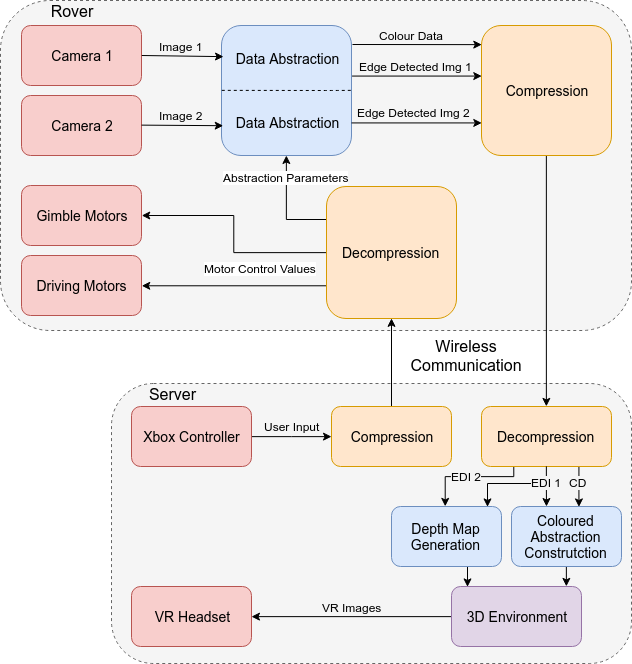
\includegraphics[width=0.9\textwidth]{Figures/System.png}
      \caption[System Overview Block Diagram]{System Overview Block Diagram.}
      \label{fig:system}
    \end{center}
\end{figure}